%-------------------------
%makefile
%(c) H.Buchmann FHNW 2014
%export TEXINPUTS=${HOME}/fhnw/edu/:${HOME}/fhnw/edu/tinL/config/latex:${HOME}/fhnw/edu/config//:
%-------------------------
\documentclass{beamer}
\usepackage{latex/beamer}
%---------------------
%local defines
%(c) H.Buchmann FHNW 2009
%$Id$
%---------------------
\newcommand{\target} {\beaglebone\xspace}
\newcommand{\targetS}{{\bf BBG}\xspace}
\newcommand{\host}   {{\em Host}\xspace}
\newcommand{\targetroot} {{\bf target-root}\xspace}
\newcommand{\kernel} {{\bf kernel}\xspace}
\renewcommand{\c}{{\bf C}\xspace}
\newcommand{\cpp}{{\bf C++}\xspace}
\newcommand{\posix}{{\bf POSIX}\xspace}

\input{/home/buchmann/latex/dirtree/dirtree.tex}

\usepackage[absolute]{textpos}
\setlength{\TPHorizModule}{1mm}
\setlength{\TPVertModule}{1mm}

\begin{document}

\newcommand{\uboot}{{U-Boot \xspace}}

\title[Assembly]{Zusammenbau\\Assembly}

\frame{\titlepage}

\begin{frame}{Um was geht es ?}{Ein erstes vollst�ndiges System}
 \begin{itemize}
  \item Bootloader \uboot
  \item \kernel
  \item \unix 
 \end{itemize}
\end{frame}

\begin{frame}{Die Schichten}
\begin{center}
 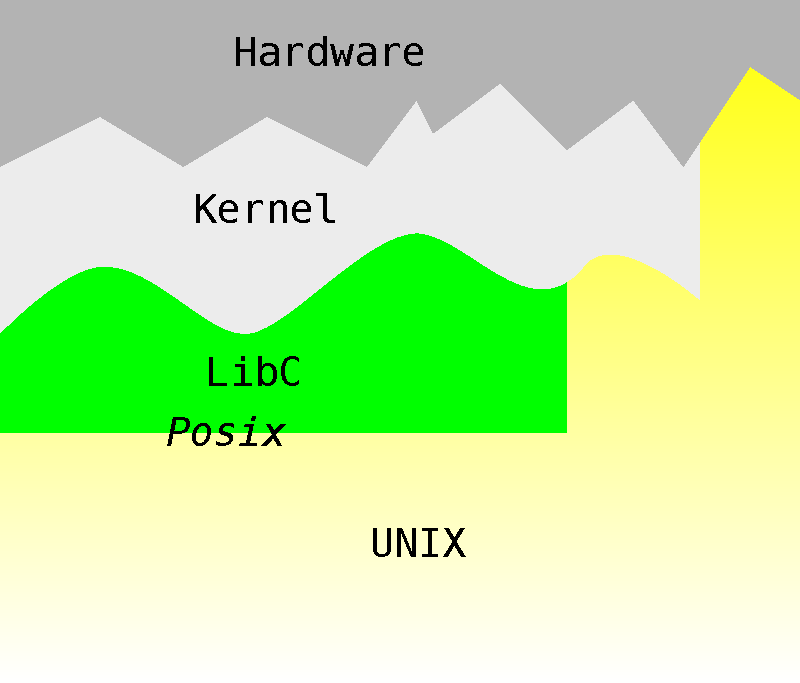
\includegraphics[width=0.75\textwidth]{../../5-kernel/doc/layers.pdf}
\end{center}
\end{frame}

\begin{frame}{Das Ziel}{f�r \targetS}
 \begin{block}{Nach dem Reset:}
 \begin{enumerate}
  \item \uboot startet \kernel
  \item \kernel startet \unix
  \item \unix 
   \begin{itemize}
    \item konfiguriert {\em ethernet �ber USB}
    \item startet \cod{ssh} Server 
   \end{itemize}
 \end{enumerate}
 \end{block}
\end{frame}

\begin{frame}{Was wir schon haben}
 \begin{description}[root Filesystem:]
  \item[Toolchain:] download
  \item[\uboot:] selber gemacht
  \item [\kernel:] selber gemacht
  \item[root Filesystem:] download
  \begin{itemize}
   \item libc/\unix
  \end{itemize} 
 \end{description}
\end{frame}

\begin{frame}{Die Partitionen und Filesysteme}
 \begin{description}
  \item[p1] bootfs:vfat $\approx 20MiB$
   \begin{itemize}
    \item \uboot
    \begin{itemize}
     \item \cod{MLO}  
     \item \cod{u-boot.img}
     \item \cod{uEnv.txt} Konfiguration
    \end{itemize}
    \item \kernel
    \begin{itemize}
      \item \cod{zImage}
	  \item \cod{am335x-boneblack-wireless.dtb}
    \end{itemize}
   \end{itemize}
  \item[p2] rootfs:ext4 $\approx 200MiB$
  \begin{itemize}
   \item \cod{etc/init.d/rcS} init-script
  \end{itemize}
 \end{description}
\end{frame}

\section{Erster Zusammenbau}
\section{U-Boot}
\begin{frame}{\url{www.denx.de/wiki/U-Boot/WebHome}}{ein typischer Bootloader für eingebettete Systeme}
 \begin{itemize}
  \item Kommandozeilen
  \item Verbindung zum \host via RS232/USB
  \begin{itemize}
   \item \host: \cod{minicom -D /dev/ttyUSB{\em N}}, $N=0,1..$
   \item 115200 Baud \cod{8N1}
   \item {\Large no} Handshaking
  \end{itemize}
  \item Kopiert Daten von
  \begin{itemize}
   \item SD-Karten
   \item Netz
  \end{itemize}
  in das Memory vom \targetS
 \end{itemize}
\end{frame}

\subsection{Bedienung}
\begin{frame}{Ein paar typische Befehle}
 \begin{itemize}
  \item \cod{help}
  \item \cod{printenv} Zeigt die Umgebung
  \item \cod{md addr} Memory display
  \item Filesysteme 
  \begin{description}
   \item[ext4] \cod{fatls mmc p}\\\cod{fatload mmc p memAddr file}
   \item[fat] \cod{fatls mmc p}\\\cod{ext4load mmc p memAddr file}
  \end{description}
  \item \cod{tftpboot [loadAddress] [[hostIPaddr:]bootfilename]} 
  \item \cod{bootz kernelAddr - fdt}
 \end{itemize}
\end{frame}


\begin{frame}{U-Boot Bedienung}{Siehe \cod{tools/u-boot-copy-paste.cmd}}
 \begin{itemize}
  \item copy paste
  \remark{kann sich ändern}
 \end{itemize}
\end{frame}


\subsection{Herstellung}

\begin{frame}{Verzeichnisstruktur}
\dirtree{%
.1 4-uboot \DTcomment{u-boot section}.
.2 tc \DTcomment{link to toolchain}.
.2 tools \DTcomment{scripts}.
.2 config \DTcomment{configuration}.
.2 build \DTcomment{home of binaries}.
.3 MLO \DTcomment{second stage bootloader}.
.3 u-boot.img \DTcomment{the U-Boot}.
}
\end{frame}

\begin{frame}{Herstellung}
 \begin{itemize}
  \item Repository \url[http]{git.denx.de/u-boot.git}
  \item Version \url{ftp.denx.de/pub/u-boot}
  \item Script \cod{tools/u-boot.sh {\em what}}
  \begin{itemize}
   \item {\em what}:\cod{am335x\_boneblack\_defconfig}, \cod{all}, \cod{help}, \cod{distclean}
  \end{itemize}
 \end{itemize}
\end{frame}

\subsection{Installation}

\begin{frame}[fragile]{SD-Karte:Partionierung}
 \begin{itemize}
  \item Partitionen: \cod{fdisk}
{\footnotesize
\begin{verbatim}  
Device         Boot Start    End Sectors  Size Id Type
/dev/mmcblk0p1 *     2048  36863   34816   17M  b W95 FAT32
/dev/mmcblk0p2      36864 299007  262144  128M 83 Linux
\end{verbatim}
}
 \item Filesysteme
 \begin{itemize}
  \item Partition 1: vfat: \cod{mkfs.vfat} für U-Boot
  \item Partition 2: ext4: \cod{mkfs.ext4}
 \end{itemize}
 \end{itemize}
\end{frame}

\begin{frame}[fragile]{Partitionen}
\begin{block}{Partition 1:Die U-Boot Files}
{\footnotesize
\begin{verbatim}
 76152 16. Okt 12:52 MLO
375952 16. Okt 12:52 u-boot.img
[end{verbatim}
}
\end{block}
\begin{block}{Partition 2:Für \linux \cod{/boot}}
{\footnotesize
\begin{verbatim}
   61957 Sep 27 16:15 am335x-boneblack-wireless.dtb
10424832 Sep 27 16:15 zImage
\end{verbatim}
}
\end{block}
\end{frame}



%-------------------------
%big-picture
%(c) H.Buchmann FHNW 2008
%export TEXINPUTS=${HOME}/fhnw/edu/:${HOME}/fhnw/edu/tinL/config/latex:${HOME}/fhnw/edu/config//:
%https://drive.switch.ch/index.php/s/xwpXAvMX91n5CtE
%-------------------------
\documentclass{beamer}
\usepackage{latex/beamer}
%---------------------
%local defines
%(c) H.Buchmann FHNW 2009
%$Id$
%---------------------
\newcommand{\target} {\beaglebone\xspace}
\newcommand{\targetS}{{\bf BBG}\xspace}
\newcommand{\host}   {{\em Host}\xspace}
\newcommand{\targetroot} {{\bf target-root}\xspace}
\newcommand{\kernel} {{\bf kernel}\xspace}
\renewcommand{\c}{{\bf C}\xspace}
\newcommand{\cpp}{{\bf C++}\xspace}
\newcommand{\posix}{{\bf POSIX}\xspace}

\input{/home/buchmann/latex/dirtree/dirtree.tex}

\title{Kernel}
\begin{document}

\frame{\titlepage}



\begin{frame}{Ziele}{Neuer \kernel auf \target}
 \begin{itemize}
  \item Download
  \item Setup
  \item Konfiguration
  \item Kompilation
  \item Installation
 \end{itemize}
\end{frame}

%-------------------------
%big-picture
%(c) H.Buchmann FHNW 2008
%$Id$
%-------------------------
\svnInfo $Id$

\title[The Big Picture]{The Big Picture\\{\tiny \svnId}}
\frame{\titlepage}

\begin{frame}{The Big Picture}
 \begin{itemize}
  \item \linux ist:
  \begin{itemize}
   \item Software mit klassischen Methoden hergestellt
   \item gross
   \item komplex {\tiny nicht kompliziert}
  \end{itemize}
  \item Darum:
  \begin{itemize}
   \item \alert{Die grundlegenden Mechanismen beachten}
   \item \alert{�bersicht bewahren}
   \item \alert{Verzeichnisstrukturen}: wo ist was.
   \end{itemize}
  \end{itemize}
\end{frame}

\begin{frame}{Ein paar Daten: zum \linux (Kernel)}
 \begin{itemize}
  \item $\approx 10M$ SLOC (Source Lines of Code)
  \item $\approx 2.3K$ Verzeichnisse
  \item $\approx 33K$ Files davon
  \begin{itemize}
   \item $\approx 30 K$ \cod{\{c$|$h\}}-Files
   \item $\approx 1 K$ Assembler Files
   \item $\approx 1.4K$ Makefiles
   \item Rest: \cod{Makefile}, Scripts etc.
  \end{itemize}
 \end{itemize}
 \begin{remarks}
  \item $M=10^6$ $K=10^3$
  \item Gemacht mit \cod{sloccount}
 \end{remarks}
\end{frame}

\section{ProgrammierSprachen}
\begin{frame}{Die ProgrammierSprachen}
 \begin{description}[Assembler]
  \item[C] 
     Unabh�ngig von Rechnerarchitektur,
     Hauptsprache f�r {\em Bootloader},{\em Kernel},{\em libc}
  \item[Assembler] F�r kleine Anpassungen
  \item[Skript] F�r Routineaufgaben
  \item[Makefile] F�r den Zusammenbau
 \end{description}
\end{frame}

\section{Tools}
\begin{frame}{Die wichtigsten Werkzeuge}
 \begin{description}
  \item[Compiler]  \cod{gcc} \url{gcc.gnu.org} 
  \item[binutils] Sammlung von Programmen\footnote{Liste nicht vollst�ndig} 
     (\url{www.gnu.org/software/binutils})
 \begin{description}
  \item[Assembler] \cod{as} 
  \item[Linker]    \cod{ld}
  \end{description}
  \item[Maker] \cod{make} \url{www.gnu.org/software/make}
 \end{description}
\end{frame}

\section{Komponenten}
\begin{frame}{Die Komponenten}
 \begin{description}[BootLoader]
  \item[BootLoader] {\em reset} Handler, SingleUser
  \item[Kernel] Prozessverwaltung,Treibersammlung
  \item[libc] Normierte (POSIX) Schnittstelle,Kernel-\unix 
  \item[\unix] Filesystem, Sammlung von Programmen und Daten
 \end{description}
\end{frame}

\begin{frame}{Die Komponenten:Eigenschaften}
 Komponenten lassen sich:
 \begin{itemize}
  \item einzeln hergestellen
  \item kombinieren 
  \item austauschen
 \end{itemize}
\end{frame}

\begin{frame}{Die Komponenten:Wo sind sie ?}
 \begin{description}[BootLoader]
  \item[BootLoader] nicht fl�chtiger Speicher: z.B. Flash
  \item[Kernel] RAM
  \item[libc] RAM
  \item[\unix] RAM,Harddisk,MemoryCard,NFS 
 \end{description}
\end{frame}

\section{Zusammenbau}
\subsection{Bestehende Systeme}
\begin{frame}{Bestehende Systeme}
 \begin{description}[openEmbedded]
  \item[openEmbedded] \url{www.openembedded.org}
  
  (\'a la Gentoo) Skriptsammlung/Repository, f�r viele
  Rechnerarchitekturen

  \item[buildroot] \url{buildroot.uclibc.org}
  
      Makefiles/patches f�r viele Rechnerarchitekturen
      
  \item[CLFS] \url{cross-lfs.org/view/clfs-embedded/arm} 
  
   {\bf C}ross-Compiled {\bf L}inux {\bf F}rom {\bf S}cratch 

   Anleitung 
 \end{description}
\end{frame}

\begin{frame}{Bestehende Systeme:Kritik}
 \begin{description}
  \item[openEmbedded/buildroot] 
  \begin{itemize}
   \item Grosse Systeme
   \item Braucht zus�tzliche {\em tools}
   \item F�hren zus�tzliche Komplikationen ein 
  \end{itemize}      
  \item[CLFS] Sehr rezeptartiger Aufbau     
 \end{description}
\end{frame}

\subsection{Unser System}
\begin{frame}{Unser System: Modifiziertes CLFS}
 Warum ?
 \begin{itemize}
  \item Basiert auf der originalen Software
  \item Die klassischen Tools (\cod{Makefile}) sind schon sehr gut
  ausgebaut.
  \item Brauchen tieferen Einblick in das ganze System
  \item Nur ein bis zwei Rechnerarchitekturen 
 \end{itemize} 
\end{frame}

\section{Aufbau der Vorlesung/Labor}
\begin{frame}{Aufbau}{\url{websvn.fhnw.ch/trac/edu/browser/linux-lab/1-current}}
 \begin{description}[2-unix-use]
  \item[0-intro] Diese Folien
  \item[1-tools] Die Werkzeuge
  \item[2-unix-use] \unix aus Benutzersicht: Host und Target
  \item[3-uboot] Wie startet ein Rechner
  \item[4-kernel] Das \linux: Konfiguration/Herstellung
  \item[5-libc] Verbindung \linux \unix
  \item[6-unix] \unix Konfiguration/Herstellung
  \item[7-build] ein {\em build}  System
 \end{description}
\end{frame}



\section{Herstellung}

\subsection{Download}
\begin{frame}{\url{github.com/beagleboard/linux}}
             {Mehrere M�glichkeiten}
 \begin{itemize}
  \item das ganze git repository
  \item nur die letzten $n$ Versionen \cod{--depth=$n$}
  \item zip File 
 \end{itemize}
\end{frame}

\subsection{Setup}
\begin{frame}{Tools}{Siehe \cod{4-devel}}
 \begin{description}[toolchain]
 
  \item[toolchain] {\small \url{sourceforge.net/projects/fhnw-tinl/files}}
   \begin{itemize}
    \item \cod{gcc-6.2.0-arm-64bit.tar.gz}
    \item Prefix: \cod{arm-linux-gnueabihf-}
    \begin{itemize}
     \item beschreibt:
     \begin{itemize}
      \item Architektur: \cod{armv7}
      \item {\bf A}pplication {\bf B}inary {\bf I}nterface: \cod{gnueabihf}
     \end{itemize}
    \end{itemize}
    \end{itemize}
  \item[make] Normales \cod{make}
  \begin{itemize}
   \item \kernel Herstellung:
   \begin{itemize}
    \item \cod{make {\em cmd}}
   \end{itemize}
  \end{itemize}
 \end{description}
\end{frame}

\begin{frame}{Wo ist was ?}
 \dirtree{%
  .1 tinL.
  .2 5-kernel.
  .3 build \DTcomment{generated kernel files}.
  .4 {.config} \DTcomment{die aktuelle Konfiguration}.
  .3 tools \DTcomment{for making}.
  .4 kernel.sh \DTcomment{wrapper to \kernel Makefile}.
  .3 config.
  .4 config.sh \DTcomment{for kernel.sh}.
  .4 kernel.config \DTcomment{'gute' kernel Konfiguration}.
  .2 resources.
  .3 beaglebone-black.
  .4 linux \DTcomment{the source tree}.
 }
\end{frame}

\subsection{Herstellung}
\begin{frame}{Erste Konfiguration}
 \begin{itemize}
  \item Hilfe
  \begin{itemize}
   \item \cod{./tools/kernel.sh help}
  \end{itemize}
  \item Vordefinierte Konfiguration
  \begin{itemize}
   \item \cod{./tools/kernel.sh bb.org\_defconfig}
  \end{itemize}
  \item Anpassung der Konfiguration
  \begin{itemize}
  \item \cod{./tools/kernel.sh menuconfig}
  \item \cod{./tools/kernel.sh xconfig}
   \end{itemize}
 \end{itemize}
\end{frame}

\begin{frame}{Kompilation}
 \begin{itemize}
  \item \cod{./tools/kernel.sh zImage}
  \begin{itemize}
   \item erzeugt  \cod{build/arch/arm/boot/zImage}
  \end{itemize} 
  \item \cod{./tools/kernel.sh dtbs}
  \begin{itemize}
   \item erzeugt \cod{build/arch/arm/boot/dts/am335x-boneblack-wl1835mod.dtb}
   {\em Devicetree} 
   \remark{{\em Devicetree} sp�ter behandelt}
  \end{itemize} 
 \end{itemize}
\end{frame}

\begin{frame}{Installation}{auf SD-Card}
 \begin{itemize}
  \item Kopiere
  \begin{description}[Devicetree]
   \item[Image] \cod{build/arch/arm/boot/zImage}
   \item[Devicetree] \cod{build/arch/arm/boot/dts/am335x-boneblack.dtb}
  \end{description}
  auf
  \begin{itemize}
   \item SD-Card {\em boot-partition}
  \end{itemize}
 \end{itemize}
\end{frame}




%\section{Startup}

\begin{frame}{Startup}{Bootloaders bei eingebetteten Systemen}
\begin{tabular}{ll|l}
 Reset $\to$ & fbl 		& {\em first stage bootloader}\\
 			 & sbc  	& ev. weitere bootloader {\em second stage bootloader}\\
			 & u-boot	& Hier haben wir Zugriff\\
			 & kernel	& Konfiguration/Parametrisierung \\
			 & linux	& 
\end{tabular}
\end{frame}

\begin{frame}{Startup}{Bootloader beim \host}
\begin{tabular}{ll|l}
 Reset $\to$ & BIOS 	& {\em first stage bootloader}\\
 			 & grub  	& {\em second stage bootloader}\\
			 & kernel	& Konfiguration/Parametrisierung \\
			 & linux	& 
\end{tabular}
\end{frame}

\subsection{U-Boot}
\begin{frame}{\url{www.denx.de/wiki/U-Boot/WebHome}}{ein typischer Bootloader für eingebettete Systeme}
 \begin{itemize}
  \item Kommandozeilen
  \item Verbindung zum \host via RS232/USB
  \begin{itemize}
   \item \host: \cod{minicom -D /dev/ttyUSB{\em N}}, $N=0,1..$
   \item 115200 Baud \cod{8N1}
   \item {\Large no} Handshaking
  \end{itemize}
  \item Kopiert Daten von
  \begin{itemize}
   \item SD-Karten
   \item Netz
  \end{itemize}
  in das Memory vom \targetS
 \end{itemize}
\end{frame}

\begin{frame}{Ein paar typische Befehle}
 \begin{itemize}
  \item \cod{help}
  \item \cod{printenv} Zeigt die Umgebung
  \item \cod{md addr} Memory display
  \item \cod{fatls mmc p}  vfat sd-card partition p
  \item \cod{fatload mmc p memAddr file}
  \item \cod{tftpboot [loadAddress] [[hostIPaddr:]bootfilename]} 
  \item \cod{bootz kernelAddr - fdt}
 \end{itemize}
\end{frame}


\begin{frame}{U-Boot Bedienung}{Siehe \cod{5-kernel/tools/u-boot.cmd}}
 \begin{itemize}
  \item copy paste
  \remark{kann sich ändern}
 \end{itemize}
\end{frame}

\subsection{Kernel}
\begin{frame}[fragile]{Übergang U-Boot-Kernel}{Bootargs}
{\scriptsize
\begin{verbatim}
 bootargs 
 'root=/dev/mmcblk0p2 rw rootdelay=1 init=linuxrc console=ttyO0,115200n8'
\end{verbatim}
}
\begin{itemize}
 \item \cod{kernel-source/Documentation/kernel-parameters.txt}
\end{itemize}
\end{frame}

\begin{frame}[fragile]{Die Kernel messages}{}
{\scriptsize
\begin{verbatim}
Starting kernel ...

Booting Linux on physical CPU 0x0
Initializing cgroup subsys cpuset
Initializing cgroup subsys cpu
Initializing cgroup subsys cpuacct
...
Kernel command line: root=/dev/mmcblk0p2 rw rootdelay=1 init=linuxrc console=ttyO0,115200n8
...
Waiting 1 sec before mounting root device...
EXT4-fs (mmcblk0p2): couldn't mount as ext3 due to feature incompatibilities
EXT4-fs (mmcblk0p2): couldn't mount as ext2 due to feature incompatibilities
EXT4-fs (mmcblk0p2): mounted filesystem with ordered data mode. Opts: (null)
VFS: Mounted root (ext4 filesystem) on device 179:2.
\end{verbatim}
}
\end{frame}


\begin{frame}{Workflow}{Notationen}
 \begin{description}[\tar]
  \item[\cod{\em sd-card}] die Partition vom rootfs auf der SD Karte
  \item[\tar] das heruntergeladene rootfs
  \item[\cod{\em target-root}] das rootfs von \targetS auf dem \host
 \end{description}
\end{frame}

\begin{frame}{Workflow}{schrittweise Verbesserung}
 \begin{enumerate}
  \item Initialer Download \tar
  \item \cod{target-root}
  \begin{itemize}
   \item \cod{tar -xf \tar\ -C {\em target-root}}
  \end{itemize} 
  \item Transfer auf \cod{\em sd-card}
  \begin{itemize}
   \item \cod{rsync -av {\em target-root}/ {\em sd-card}/}
   \item \cod{sync} 
  \end{itemize} 
  \item Test/Konfiguration auf dem \targetS
  \item Update auf dem \host
  \begin{itemize}
   \item \cod{rsync -av {\em sd-card}/ {\em target-root}/}
  \end{itemize} 
  \item $\to$ 4
 \end{enumerate}
\end{frame}

\begin{frame}{Die Files}
 \begin{block}{Partition 1: vfat}
  \begin{itemize}
   \item \cod{MLO}
   \item \cod{u-boot.img}
  \end{itemize}
 \end{block}
% \vspace{-4mm}
 \begin{block}{Partition 2: ext4}
  \begin{itemize}
   \item rootfs auf dem \host
   \item \cod{rsync -av target-root/ {\em sd-card/}}
   \item \cod{sync}
   \item \cod{/boot/zImage}
   \item \cod{/boot/am335x-boneblack-wireless.dtb}
  \end{itemize}
 \end{block}
 
\end{frame}



%\section{}
%\begin{frame}{Start}{auf \target}
% \begin{itemize}
%  \item u-boot
%  \begin{itemize}
%   \item UART-USB Kabel
%  \end{itemize}
%  \begin{itemize}
%   \item Befehle in \cod{scripts/u-boot.cmd}
%  \end{itemize}
% \end{itemize}
%\end{frame}

\section{Aufgaben}

\begin{frame}{Ziel}
 \begin{itemize}
  \item \cod{hello-world} auf dem \host und auf dem \targetS
  \item \cod{primes} auf dem \host und auf dem \targetS
 \end{itemize}
\end{frame}


\begin{frame}{The big Picture}
 \begin{itemize}
  \item Source File: \cod{hello-world.cc}
  \item falls es nicht klapt ?
  \begin{itemize}
   \item wo ist der File ?
  \end{itemize}
 \end{itemize}
\end{frame}


%\subsection{Die Programme}
%\begin{frame}{Development}{\cod{hello-world-c.c}}
%\hspace*{-8mm}
%{
%\begin{tabular}{llllll}
% Host & Target & OS & Toolchain & Verbindung & Bemerkungen\\
% \hline
% \targetS & \targetS & Debian & mitgeliefert&&\\
% \host   & \targetS & Debian & \cod{\tiny tc-tinl-gcc-8.1.0-2018.05.21.tar.gz} & sshfs\\
% \host   & \targetS & minimal & \cod{\tiny tc-tinl-gcc-8.1.0-2018.05.21.tar.gz} & SD-Card  &später\\
% \host   & \targetS & minimal & \cod{\tiny tc-tinl-gcc-8.1.0-2018.05.21.tar.gz} & curlftpfs&später\\
%\end{tabular}
%}
%\remark{Toolchain auf der Cloud: \href{https://drive.switch.ch/index.php/s/A6H382zEGDrgfAL}
%       {\Huge tinL}}
%\end{frame}


\end{document}



\subsection{RootFS}
\begin{frame}{Init Script}{\cod{target-root-{\em version}.tar.gz}}
 \begin{itemize}
  \item \cod{/etc/init.d/rcS} das {\em Init-Script}
  \item \cod{ifconfg} f�r Internet
  \item \cod{sshd} Server f�r Verbindung
 \end{itemize}
\end{frame}


\begin{frame}{Workflow}{Notationen}
 \begin{description}[\tar]
  \item[\cod{\em sd-card}] die Partition vom rootfs auf der SD Karte
  \item[\tar] das heruntergeladene rootfs
  \item[\cod{\em target-root}] das rootfs von \targetS auf dem \host
 \end{description}
\end{frame}

\begin{frame}{Workflow}{schrittweise Verbesserung}
 \begin{enumerate}
  \item Initialer Download \tar
  \item \cod{target-root}
  \begin{itemize}
   \item \cod{tar -xf \tar\ -C {\em target-root}}
  \end{itemize} 
  \item Transfer auf \cod{\em sd-card}
  \begin{itemize}
   \item \cod{rsync -av {\em target-root}/ {\em sd-card}/}
   \item \cod{sync} 
  \end{itemize} 
  \item Test/Konfiguration auf dem \targetS
  \item Update auf dem \host
  \begin{itemize}
   \item \cod{rsync -av {\em sd-card}/ {\em target-root}/}
  \end{itemize} 
  \item $\to$ 4
 \end{enumerate}
\end{frame}

\begin{frame}{Die Files}
 \begin{block}{Partition 1: vfat}
  \begin{itemize}
   \item \cod{MLO}
   \item \cod{u-boot.img}
  \end{itemize}
 \end{block}
% \vspace{-4mm}
 \begin{block}{Partition 2: ext4}
  \begin{itemize}
   \item rootfs auf dem \host
   \item \cod{rsync -av target-root/ {\em sd-card/}}
   \item \cod{sync}
   \item \cod{/boot/zImage}
   \item \cod{/boot/am335x-boneblack-wireless.dtb}
  \end{itemize}
 \end{block}
 
\end{frame}




\section{Wi-Fi}
\begin{frame}{Ziele}{Wi-Fi}
 \begin{itemize}
  \item Konfiguration: \kernel
  \item Neues root-fs: download
  \item Konfiguration: wi-fi Zugang
  \item schrittweises Vorgehen
 \end{itemize}
\end{frame}

\subsection{Kernel}

\begin{frame}{Kernel}{Konfiguration}
{\footnotesize
 \dirtree{%
 .1 Kernel Configuration.
 .2 Networking support.
 .3 Wireless.
 .4 <*> cfg80211 - wireless configuration API.
 .4 <*> Generic IEEE 802.11 Networking Stack (mac80211).
 .2 Device Drivers.
 .3 Network device support.
 .4 Wireless LAN.
 .5 <*> TI wl18xx support.
 .5 <*> TI wlcore SPI support.
 .5 <*> TI wlcore SDIO support.
 }
}
\vspace{-5mm}
\begin{block}{Resultate}
 \begin{itemize}
  \item \cod{dmesg | grep wl}
 \end{itemize}
\end{block}
\end{frame}

\begin{frame}{Firmware}{Weitere Konfiguration}
 {\footnotesize
 \dirtree{%
 .1 Kernel Configuration.
 .2 Device Drivers.
 .3 Generic Driver Options.
 .4 [*] Include in-kernel firmware blobs in kernel binary.
 }
}
\vspace{-5mm}

\begin{block}{Resultate}
 \begin{itemize}
  \item \cod{dmesg | grep wl}
  \item \cod{ip link set wlan0 up}
  \item \cod{iw wlan0 scan}
  \item Weitere Konfiguration
 \end{itemize}
\end{block}
\end{frame}

\subsection{Connect}
\begin{frame}[fragile]{wpa}
 \begin{itemize}
  \item \cod{wpa\_passphrase}
  \item eduroam Versuch
{\footnotesize
\begin{verbatim}
network={
  ssid="eduroam"
  key_mgmt=WPA-EAP
  identity="hans.buchmann@fhnw.ch"
  domain_suffix_match="welcome.fhnw.ch"
  phase2="auth=MSCHAPV2"
  password="----"
}
\end{verbatim}
}
 \end{itemize}
\end{frame}

\begin{frame}[fragile]{DHCP}
 \begin{block}{manuell}
  \begin{itemize}
   \item \cod{udhcpc -v -i wlan0}
   \item \cod{ifconfig wlan0 {\em ip}}
   \begin{itemize}
    \item \cod{\em ip} abgelesen von \cod{udhcpc -v -i wlan0}
   \end{itemize}
  \end{itemize}
 \end{block}
 \begin{block}{automatisch/callback}
\vspace{-3mm}
{\tiny
\begin{verbatim}
#!/bin/sh
#---------------------
#on-udhcpc.sh
#(c) H.Buchmann FHNW 2017
#---------------------
case ${1} in
 defconfig)
  echo defconfig------- ${interface} ${ip};;
  bound)
   ifconfig ${interface} ${ip};;
esac
\end{verbatim}
}
\end{block}
\end{frame}

\begin{frame}{route/dns}
\begin{itemize}
 \item route
 \begin{itemize}
  \item \cod{route add default gw {\em gw-ip} wlan0}
 \end{itemize}
 \item DNS
 \begin{itemize}
   \item \cod{/etc/resolv.conf}
 \end{itemize}
\end{itemize}
\end{frame}



\section{Aufgaben}
\begin{frame}{Aufgabe}
 \begin{description}
%  \item[\uboot] Automatisches booten: \cod{uEnv.txt}
  \item[\kernel] Ethernet �ber USB
  \item[\unix] Automatisches starten: \cod{/etc/init.d/tcS}
  \begin{itemize}
   \item Internet:\cod{ifconfig}
   \item ssh Server: \cod{sshd}
  \end{itemize}
  \item[wi-fi]
   \begin{itemize}
    \item \kernel firmware
    \item \unix wpa
   \end{itemize}
 \end{description}
\end{frame}

\subsection{sshd}
\begin{frame}{Ein paar tools}
 \begin{itemize}
  \item \cod{touch} - change file timestamps
  \item \cod{chown} - change file owner and group
 \end{itemize}
\end{frame}

\begin{frame}{sshd}
\begin{itemize}
 \item sshd re-exec requires execution with an absolute path
 \item Privilege separation user sshd does not exist
 \item create group \cod{root}
 \begin{itemize}
  \item \cod{addgroup -g 0 -S root} 
 \end{itemize}
 \item create user \cod{root}
  \begin{itemize}
   \item \cod{adduser -h /home/root/ -s /bin/sh -G root -S -u 0 root}
  \end{itemize}
\item create group/user \cod{sshd}
 \begin{itemize}
  \item \cod{addgroup sshd}
  \item \cod{adduser -D -H -G sshd sshd}
  \end{itemize}
\item create key
 \begin{itemize}
  \item \cod{ssh-keygen -t rsa -f /etc/ssh\_host\_rsa\_key}
 \end{itemize}
 \item File \cod{/var/empty} geh�rt root
 \item File \cod{/etc/sshd\_config}
 \begin{itemize}
  \item \cod{PermitRootLogin yes}
 \end{itemize}
\end{itemize}
\end{frame}


\end{document}
